% This template mostly comes from Xuezhen Wang. 
% And his Page is here:
%  https://www.overleaf.com/latex/templates/cityu-of-hong-kong-beamer/kygnjxtcngtg
% The latest HHU slice is modified by Xianpu Ji.
%-------------------------------------------------------------
\documentclass[10pt]{beamer}
\usepackage{tikz} % 用于位置控制
\usetikzlibrary{shapes, positioning,shadings}
\usepackage[utf8]{inputenc}
\usepackage{xeCJK}
\usepackage{graphicx}
\usepackage {mathtools}
\usepackage{utopia} %font utopia imported
\usetheme{CambridgeUS}
\usecolortheme{dolphin}
\usepackage{ctex, hyperref}
\usepackage[T1]{fontenc}
\usepackage[dvipsnames]{xcolor}
% other packages
\usepackage{latexsym,amsmath,xcolor,multicol,booktabs,calligra}
\usepackage{graphicx,pstricks,listings,stackengine}
% set colors
\definecolor{myNewColorA}{RGB}{173, 216, 230}  % 浅蓝色(蓝白色)
\definecolor{myNewColorB}{RGB}{135, 206, 235}  % 天蓝色
\definecolor{myNewColorC}{RGB}{240, 248, 255}  % 蓝白色的浅色调

\setbeamercolor*{palette primary}{bg=myNewColorC}
\setbeamercolor*{palette secondary}{bg=myNewColorB, fg = white}
\setbeamercolor*{palette tertiary}{bg=myNewColorA, fg = white}
\setbeamercolor*{titlelike}{fg=myNewColorA}
\setbeamercolor*{title}{bg=myNewColorA, fg = white}
\setbeamercolor*{item}{fg=myNewColorA}
\setbeamercolor*{caption name}{fg=myNewColorA}
\usefonttheme{professionalfonts}
% \usepackage{natbib}
% \usepackage{hyperref}

\xdefinecolor{hhucolor}{RGB}{100,195,213} % 设置背景颜色
\xdefinecolor{hhucolor2}{RGB}{173, 216, 230}
\setbeamercolor{footline}{bg=hhucolor}
\setbeamercolor{frametitle}{bg=hhucolor,fg=white}
\setbeamercolor{title}{bg=myNewColorC} % 设置标题的背景颜色
\setbeamerfont{frametitle}{size=\small}
% \setbeamercolor{frametitle}{bg=white, fg=black}

%------------------------------------------------------------
\titlegraphic{\hfill
\includegraphics[height=1.cm]{fig/HHU_logo.png}}


\setbeamerfont{title}{size=\large}
\setbeamerfont{subtitle}{size=\small}
\setbeamerfont{author}{size=\small}
\setbeamerfont{date}{size=\small}
\setbeamerfont{institute}{size=\small}
\useinnertheme{circles} % 设置目录小标题的形状
% 设置footline
\setbeamertemplate{footline}[frame number] % 只在正文中显示footline

\setbeamertemplate{navigation symbols}{}
\setbeamertemplate{headline}{}

\subtitle{\textcolor{gray}{\\2023级博士研究生开题答辩}}
\title{\textcolor{black}{\textbf{这里可以写你的论文名称}}}

\author{汇报人:简谱学记} % 汇报人
\institute{
 \\指导老师: 写你的导师
}
% \date{2025年4月8日}
% \setbeamertemplate{section page}{
%   \centering
%   \begin{beamercolorbox}[sep=12pt,center]{section title}
%     \usebeamerfont{section title}\insertsection\par
%   \end{beamercolorbox}
% }

%------------------------------------------------------------
% 修复列表项对齐

\begin{document}
\kaishu
%The next statement creates the title page.

\begin{frame}[plain]
 % 使用 tikz 绘制顶部蓝条
\begin{tikzpicture}[remember picture,overlay]
    \fill[myNewColorA] (current page.north west) rectangle ([xshift=0.5\paperwidth, yshift=-0.3cm]current page.north west);
    \fill[myNewColorB] ([xshift=0.5\paperwidth, yshift=0cm]current page.north west)
                    rectangle ([yshift=-0.3cm]current page.north east);
    % 底部横条
    % \fill[myNewColorA] (current page.south west) rectangle ([yshift=0.25cm]current page.south east);
\end{tikzpicture}
  \vspace{2.5cm}  % 调整标题和作者信息的偏移量
  \maketitle
\end{frame}

%% 设置页码
\setbeamertemplate{footline} 
{%
  \begin{beamercolorbox}[colsep=1.5pt]{upper separation line foot}
  \end{beamercolorbox}

  \begin{beamercolorbox}[ht=2.5ex,dp=1.125ex,%
      leftskip=.1cm,rightskip=.1cm plus1fil]{title in head/foot}%
      {\usebeamerfont{title in head/foot}\insertshorttitle}%
      \hfill%
      {\usebeamerfont{frame number}\usebeamercolor[black]{frame number}\insertframenumber/\inserttotalframenumber}
    \end{beamercolorbox}%
}



% Slide 1
%% 显示目录 
%% 显示目录 
\begin{frame}{目录}
    \centering
    % 设置字体大小
    \setbeamerfont{section in toc}{size=\Large} % 修改章节字体大小
    \setbeamerfont{subsection in toc}{size=\Large} % 修改子章节字体大小
    
    \tableofcontents[
        sectionstyle=show,
        subsectionstyle=show/shaded/hide,
        subsubsectionstyle=show/shaded/hide
    ]
\end{frame}



%------------------------------------------------------------

\section{研究意义}

\begin{frame}{CCEWs与热带降水变化}
    \begin{columns}[c]
        \column{0.52\textwidth}
        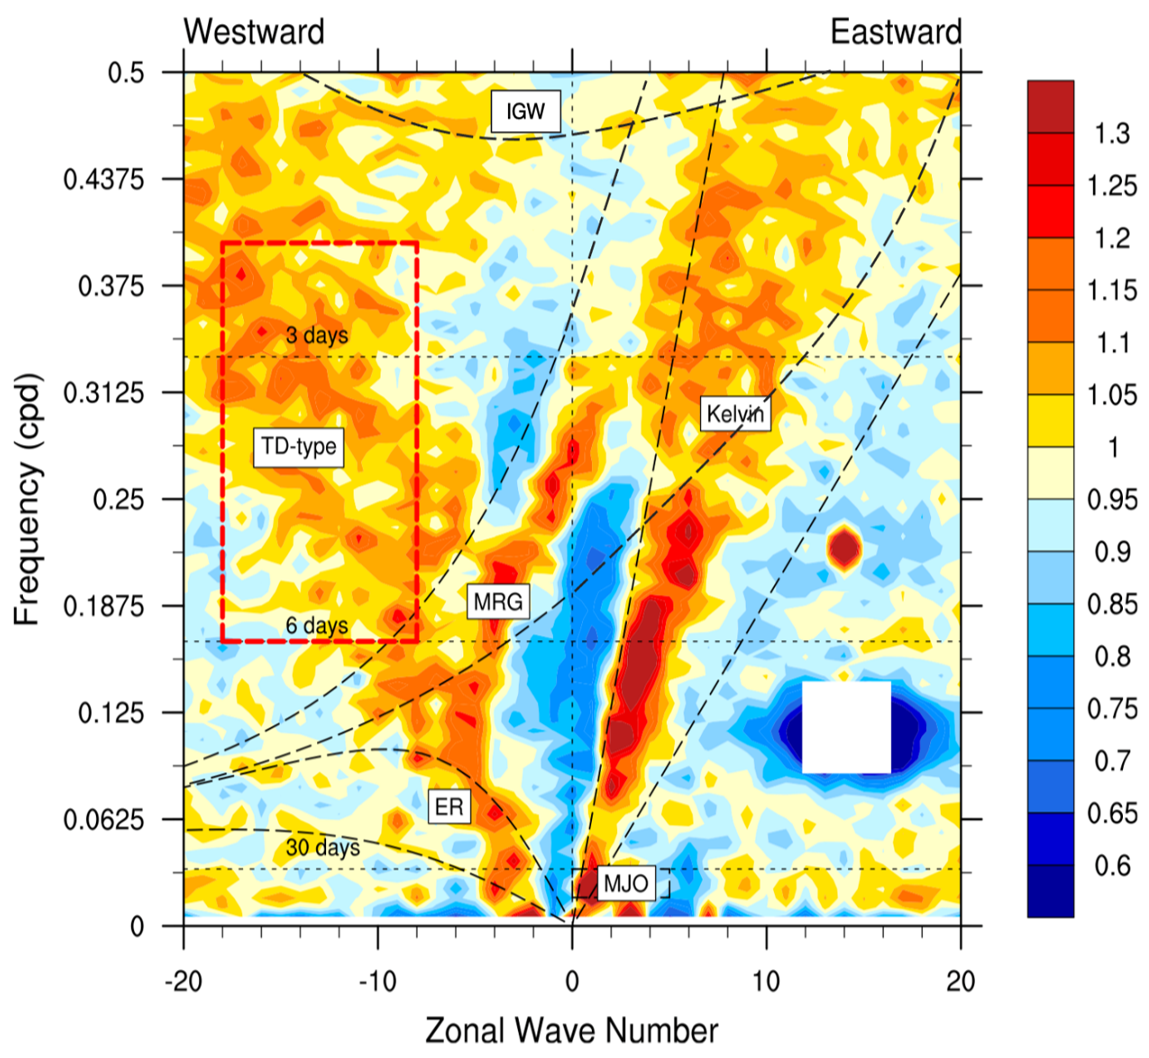
\includegraphics[width=\linewidth]{fig/spectrum.png}
        \centering {\tiny (Feng et al. 2016)}

        \column{0.48\textwidth}
        \small
        \textbf{CCEWs通过与对流的耦合,在热带降水变率中发挥重要作用}
        \vspace{0.3cm}

        \begin{itemize}
            \item $\omega^2 - k^2 - \frac{k}{\omega} = 2n + 1$
            \item $k$ 大,短波;反之为长波
            \item $\omega$ 大,高频波;反之为低频波
            \item 相速度为斜率 $\omega/k$
            \item 群速度为切线斜率 $\frac{d\omega}{dk}$
            \item IGW(高频、低频共存,东/西传)
            \item \textcolor{cyan}{Kelvin波}(非相散,东传)
            \item Rossby波(短波近似低频,西传)
            \item MRG波(高频东传,能量西传)
        \end{itemize}
    \end{columns}
\end{frame}


\section{研究现状}

\begin{frame}{{1.这里写一些小标题 } \hfill 这里写一些关键词}
    \begin{minipage}[t]{0.48\linewidth}
        \centering
        
\includegraphics[width=\linewidth]{fig/college.png} % 未来图
        \vspace{0.2cm}

        \scriptsize
        \textbf{这里描述图片的内容不是吗} \\
         \\
        
    \end{minipage}
    \hfill
    \begin{minipage}[t]{0.48\linewidth}
        \centering
        
\includegraphics[width=1\linewidth]{fig/college_no_white.png} % 历史图
        \vspace{0.2cm}
            
        \scriptsize
        \textbf{这里描述图片的内容不是吗}
        
    \end{minipage}
\end{frame}




\section{研究内容}
\begin{frame}{\textbf{这里写一些小标题}}
    \centering
    \hspace*{-0.6em}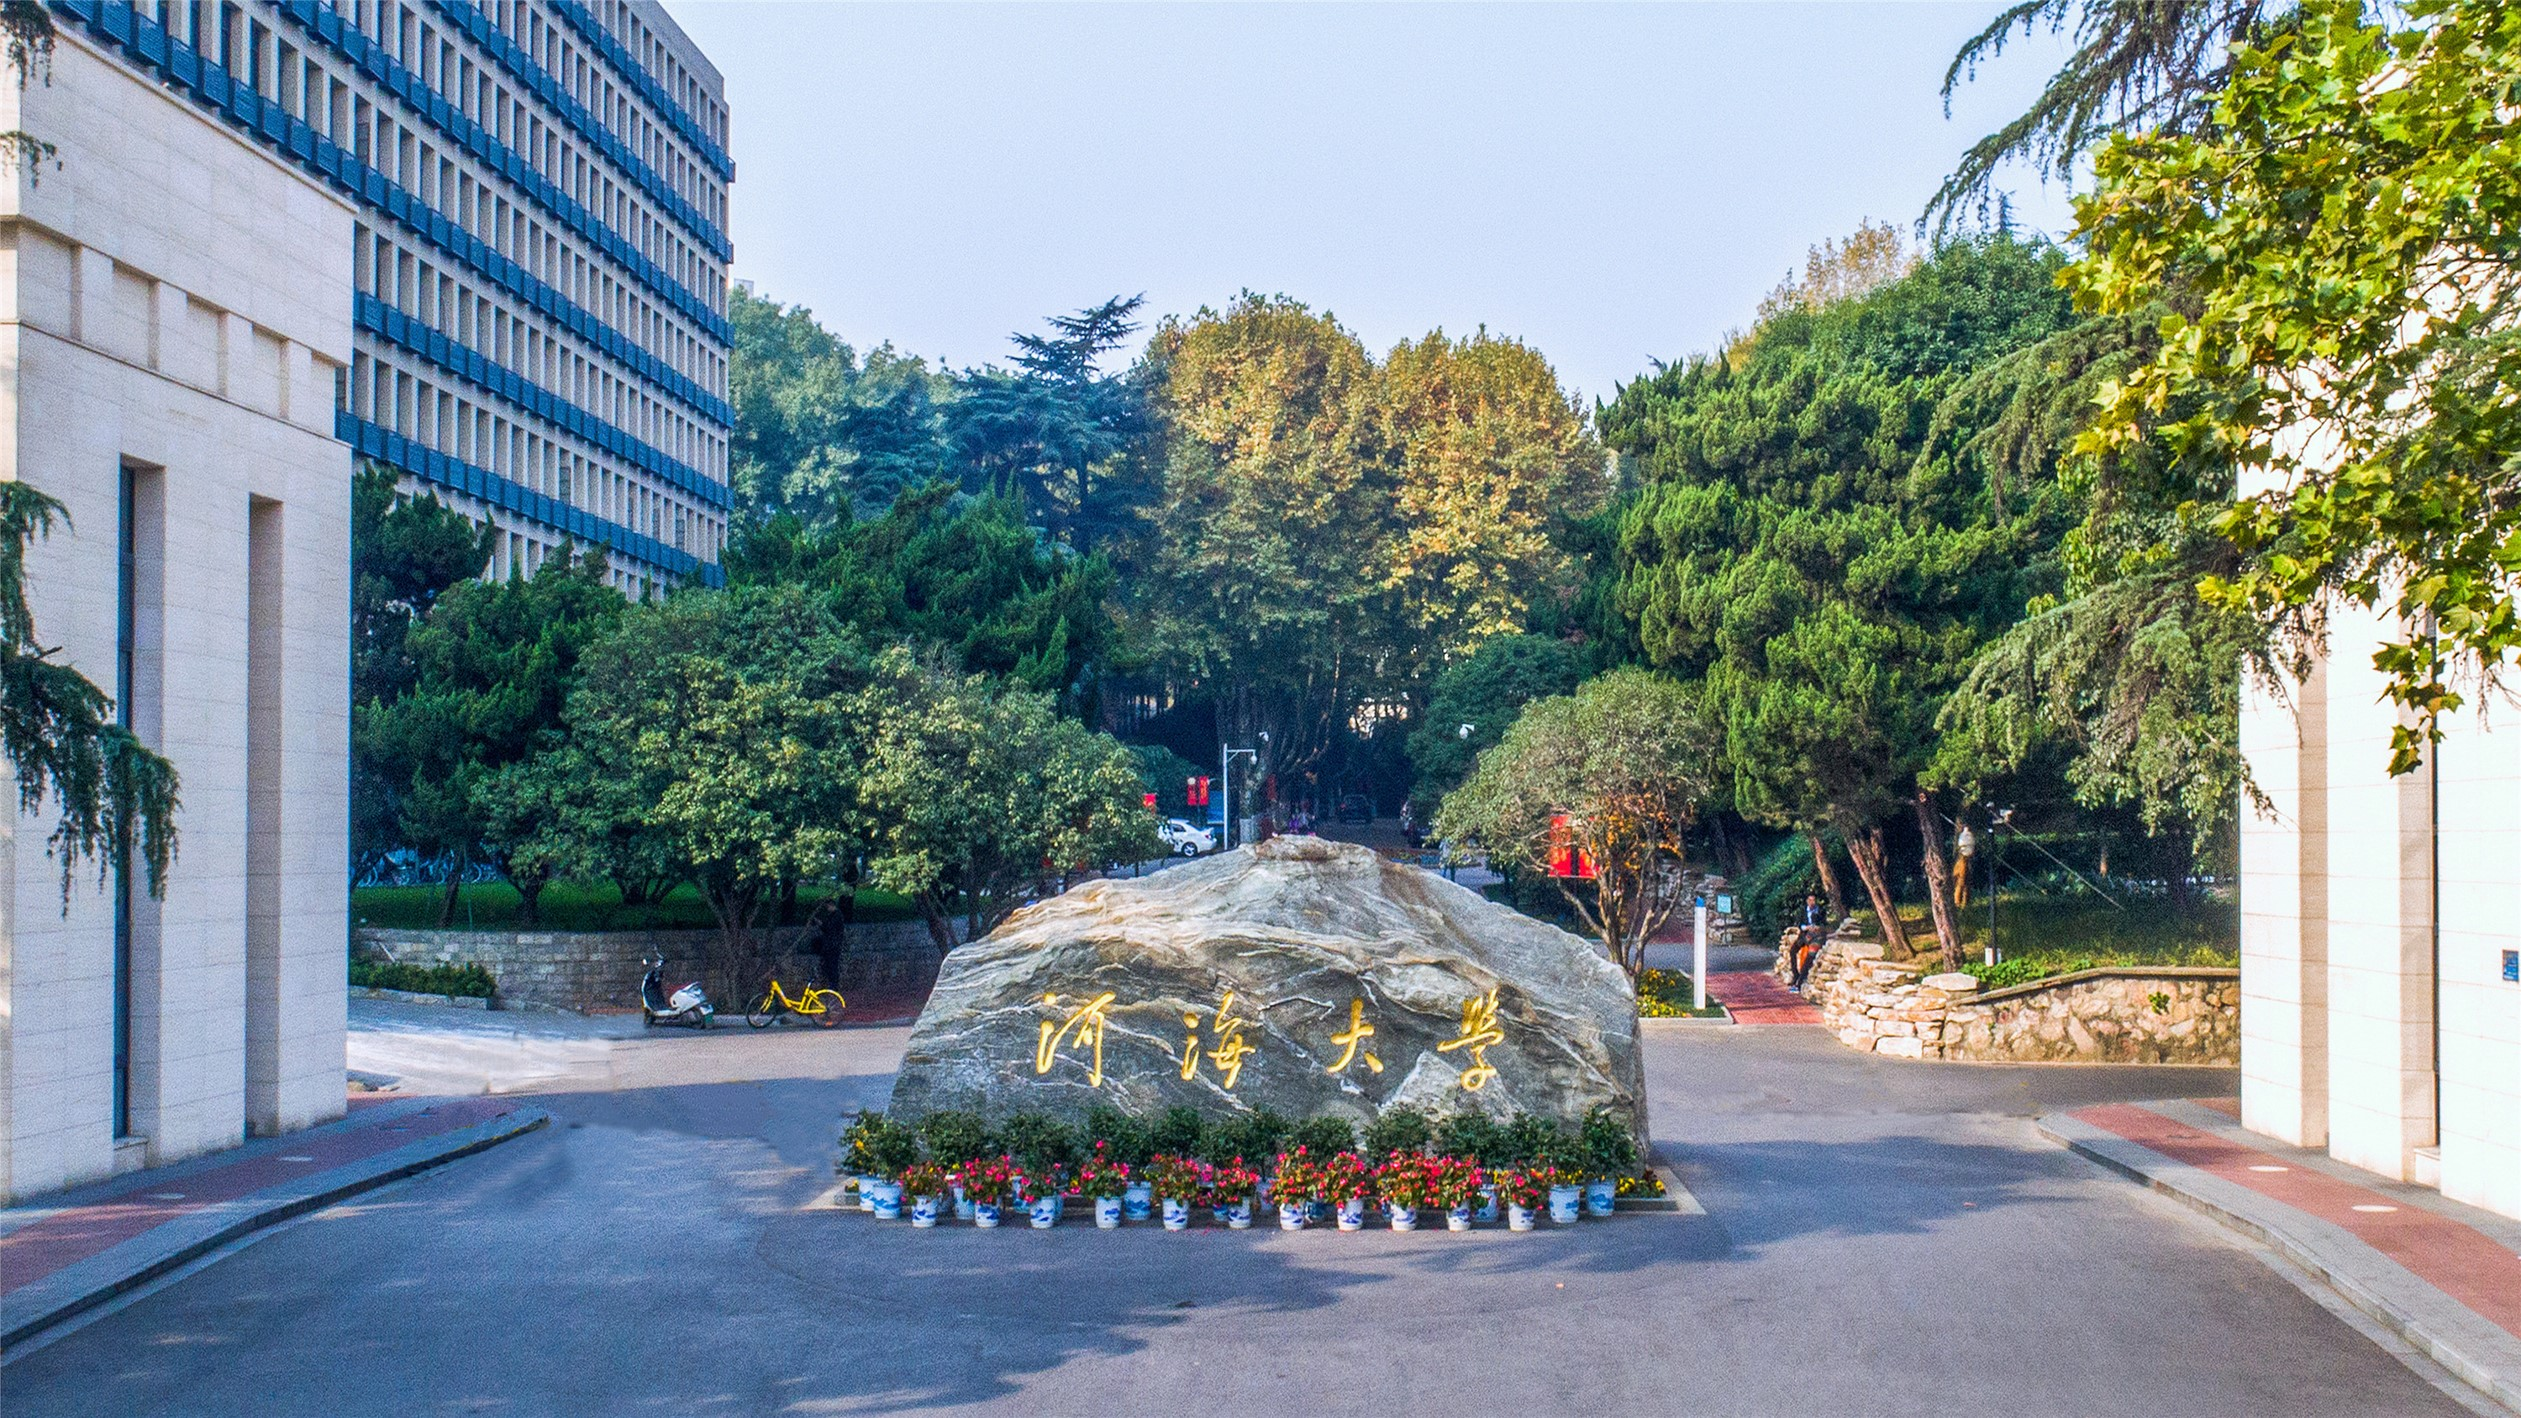
\includegraphics[width=1.05\linewidth]{fig/fengmian.jpg}
    
    % \vspace{0.1cm}
   
    \begin{itemize}
        \setlength\itemsep{0.5em}
        \setlength\leftmargini{0.1cm}
       \item \hspace*{-0.5em}这里描述图片的内容不是吗:\mbox{\textcolor{RoyalBlue}{CCKWs \textbf{这里描述图片的内容不是吗}}}
    \end{itemize}
\end{frame}



\section{计划进度}
\begin{frame}
    \begin{itemize}
        \item 一月:完成文献调研
        \item 二月:吃点好的
        \item 三、四月:早点睡觉
        \item 五月:论文撰写
    \end{itemize}
\end{frame}

\section{参考文献}

% \begin{frame}[allowframebreaks]
%     \bibliography{ref}
%     \bibliographystyle{alpha}
%     % 如果参考文献太多的话,可以像下面这样调整字体:
%     % \tiny\bibliographystyle{alpha}
% \end{frame}



\section*{Acknowledgement}  
\begin{frame}
\textcolor{myNewColorA}{\Huge{\centerline{Thank you!}}}
\end{frame}

\end{document}



